\documentclass[11pt,a4paper]{ivoa}
\input tthdefs
\input gitmeta
\usepackage[textsize=small,textwidth=3.8cm]{todonotes}

\title{Authentication for Non-Browser Clients in the VO}

% see ivoatexDoc for what group names to use here; use \ivoagroup[IG] for
% interest groups.
\ivoagroup{Distributed Services and Protocols}

\author{Patrick Dowler}
\author{Mark Taylor}
\author{Sara Bertocco}

\editor{Sara Bertocco}

% \previousversion[????URL????]{????Concise Document Label????}
\previousversion{This is the first public release}

\newcommand{\rfc}[1]{RFC\,#1}
\newcommand{\header}[1]{{\tt #1}}

\begin{document}

\begin{abstract}
Some, though not all, services in the Virtual Observatory are
restricted to users who have been authenticated and are authorized to use them.
This situation is far from unique to the VO,
and there is much industry-standard technology to manage authentication.
However, it largely assumes that authenticating clients,
often browser-based, have prior knowledge about
how authentication is to be done
for the particular service being accessed.
This document addresses a problem apparently not covered
by existing internet standards, namely how a VO client,
when pointed at a compliant VO service,
can discover authentication requirements specific to that service
and use the corresponding mechanisms to supply user credentials,
without requiring out-of-band information.
\end{abstract}


\section*{Acknowledgments}

\textcolor{red}{Editor's note: this section has to be
updated/rewritten. Authors who have someone to thank should
add here acknowledgments}
This document derives from discussions among the Grid and Web Services
working-group of IVOA. It is particularly informed by prototypes built
by Mark Taylor (University of Bristol) and Patrick Dowler
(Canadian Astronomy Data Centre).


\section*{Conformance-related definitions}

The words ``MUST'', ``SHALL'', ``SHOULD'', ``MAY'', ``RECOMMENDED'', and
``OPTIONAL'' (in upper or lower case) used in this document are to be
interpreted as described in IETF standard RFC2119 \citep{std:RFC2119}.

The \emph{Virtual Observatory (VO)} is a
general term for a collection of federated resources that can be used
to conduct astronomical research, education, and outreach.
The \href{https://www.ivoa.net}{International
Virtual Observatory Alliance (IVOA)} is a global
collaboration of separately funded projects to develop standards and
infrastructure that enable VO applications.


\section{Introduction}\label{sec:intro}

Historically many services in the VO have operated primarily or
entirely in anonymous mode.
However authentication and associated authorization
are becoming increasingly necessary in the VO,
for instance to manage data rights and as an operational necessity for
auditing and limiting service usage in the era of science platforms.
% Some way to manage authentication for VO services is therefore necessary
% but not covered in all contexts by existing industry-standard machinery.

Where the client is browser-based
it is often possible to integrate information about the authentication
methods required with the web page or web application through which
it is accessed.
\todo{is this true?  I don't understand browser-based authentication
      or what makes it work all that well}

But a desktop VO client such as Aladin, TOPCAT or Python
typically interacts with VO services differently, in one of two
ways:
\begin{enumerate}
\item Search the registry for a service, then make VO-compliant
      requests to that service (e.g.\ TAP)
\item Be presented with a URL, then retrieve the data from that URL
      (e.g.\ DataLink)
\end{enumerate}
In the first, TAP-like, case additional information is available to the
client in the form of the Registry record for the service in question,
as defined by VOResource and its service-specific extensions.
This could in principle contain metadata describing the authentication
method along with any required ancillary information such as
login endpoints.
Even if only the TAP service URL is available
(for instance because the user has typed it in rather than acquired it
from a Registry search) the VOSI Capabilities endpoint can be reliably
located ({\tt /capabilities} is a sibling of {\tt /sync} in TAP),
so that relevant VOResource information could be retrived from the VOSI
Capabilities document supplied by the service.

However in the second, DataLink-like, case
there is no information about where to find a corresponding
registry record or VOSI document,
or even a guarantee or likelihood that such a record exists.
The URL in question may not even have come from a DataLink query,
it could simply be a pointer to a protected resource like a
FITS file or VOTable in a secured filestore.
Such a URL may have been acquired from a VO query in the application
wishing to dereference it, in which case some authentication context
may be available,
but it may equally be read from a VOTable transmitted by SAMP
or saved in an earlier session, or obtained from an unrelated application;
in other words the application requiring the resource at a URL may
have no information about the VO service which produced that URL.
Then the only opportunity to acquire information about how to authenticate
is by examining the URL itself, or by HTTP communications with that URL.

The HTTP Basic Authentication method (\rfc{7617}) can be used in this scenario,
since all negotiation involving user credentials ---
request and supply of username and password ---
is done directly
over the HTTP connection from which the resource is requested.
More modern/secure/flexible authentication methods however tend to
rely on additional interaction with other, unspecified, endpoints
prior to the request itself.  For instance OAuth requires presentation
of a bearer token to retrieve protected resources from a given URL,
but there is no way given only that URL to determine where to find
such endpoints or the details of how to acquire a token from them;
in a typical OAuth usage scenario such information is known up front
by the components making the request.

No industry standard mechanism appears to exist to solve this problem.
This document therefore proposes some VO-standard mechanisms for
acquiring all the information a desktop application requires
to manage exchange of user credentials for authenticated access,
given only the URL for a suitably compliant protected resource.

The intent of this proposal is not to define new authentication
mechanisms parallel to pre-existing standards, but to provide
missing components that facilitate use from typical VO contexts
of such existing standards.

Its approach is to define some VO-specific authentication schemes
for use with the \header{WWW-Authenticate} header defined by
\rfc{9110} Section 11 (which obsoletes the earlier \rfc{7235}).
The proposal is aligned as much as possible with standard web
technology, requiring only some custom authentication schemes
which can direct the client to use existing standard authentication
mechanisms.

Given that the registry record can only be discovered for some
(TAP-like) and not other (DataLink-like) authentication scenarios,
it is no longer recommended to base discovery of authentication methods
on the {\tt securityMethod} element
defined by VOResource, as described by SSO 2.0.
Instead, the proposal here is recommended for both TAP-like and DataLink-like
scenarios.

Authenticated services in the VO are not required to use any of the  
mechanisms proposed in this document; if they can establish the
client interoperability they require using other mechanisms
they are free to do so.

\subsection{Role within the VO Architecture}

\begin{figure}
\centering

% As of ivoatex 1.2, the architecture diagram is generated by ivoatex in
% SVG; copy ivoatex/archdiag-full.xml to role_diagram.xml and throw out
% all lines not relevant to your standard.
% Notes don't generally need this.  If you don't copy role_diagram.xml,
% you must remove role_diagram.pdf from SOURCES in the Makefile.

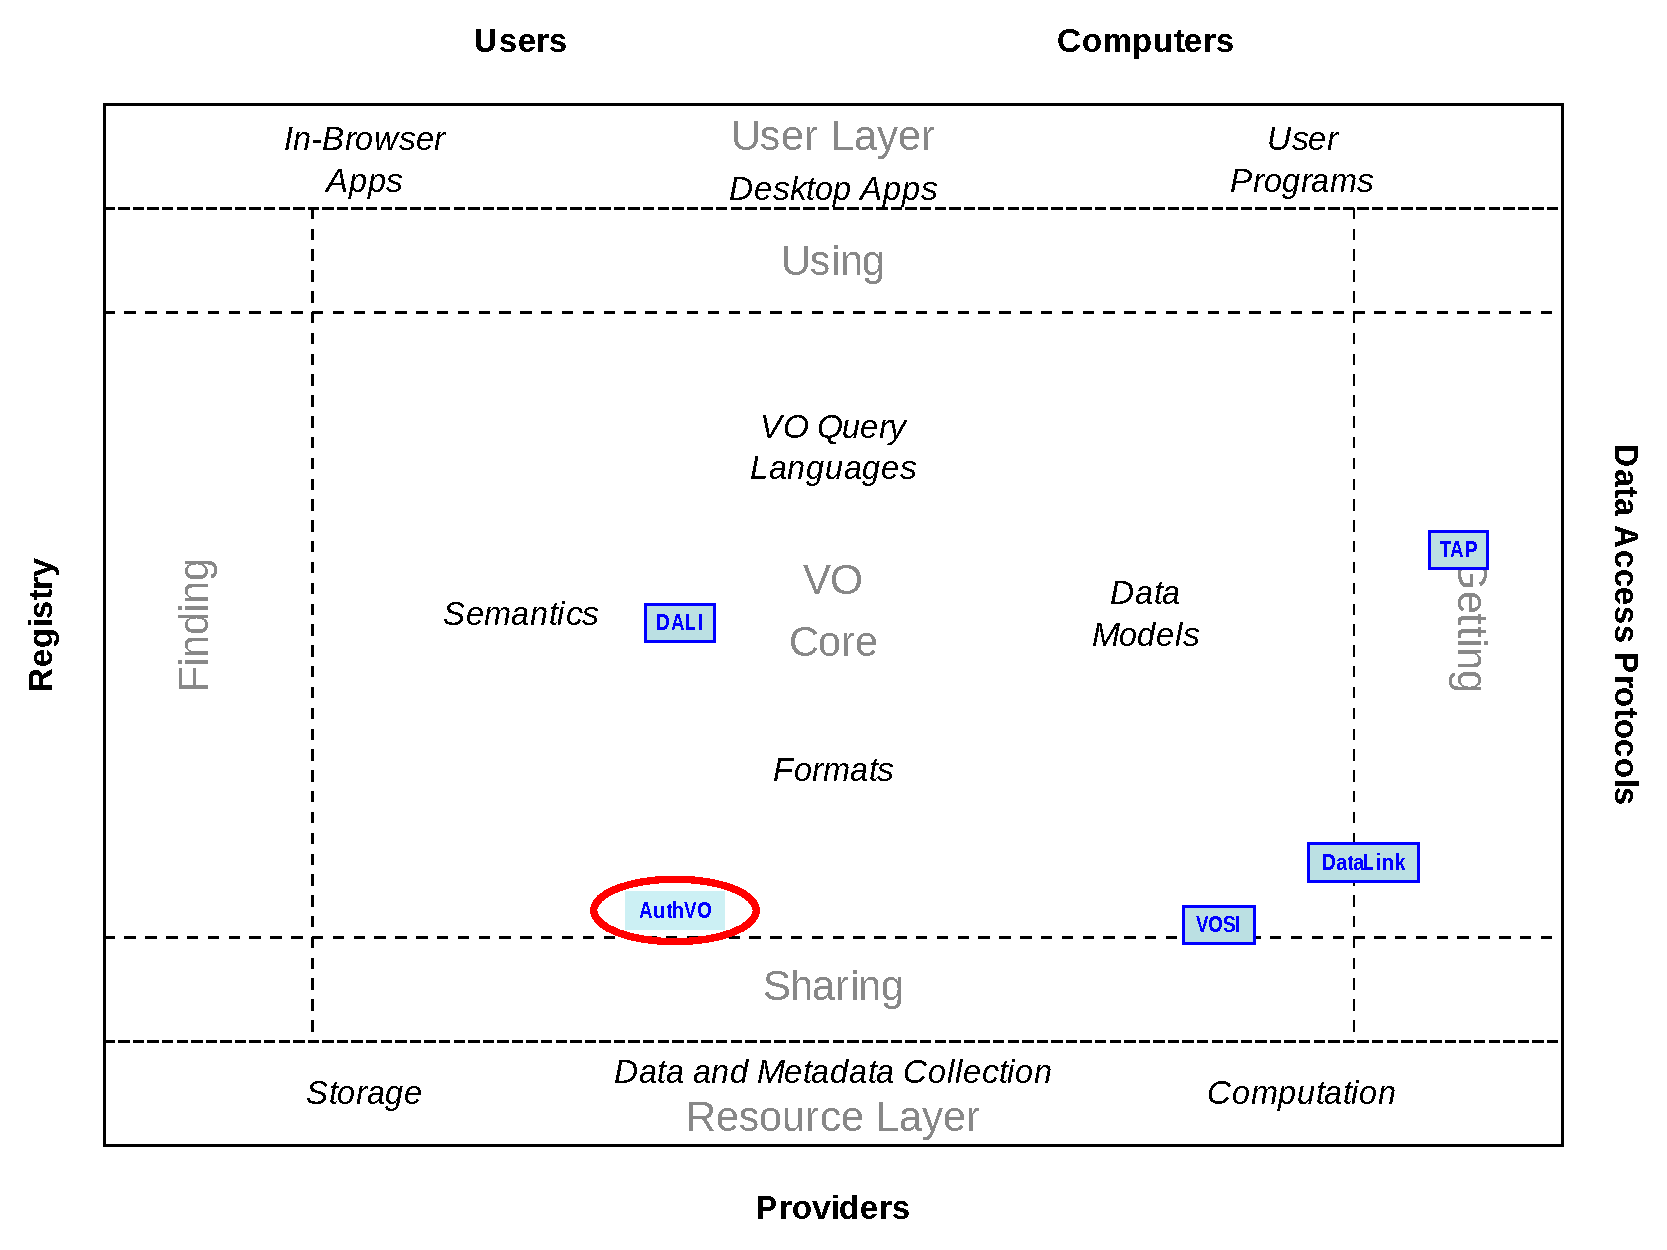
\includegraphics[width=0.9\textwidth]{role_diagram.pdf}
\caption{Architecture diagram for this document}
\label{fig:archdiag}
\end{figure}

Fig.~\ref{fig:archdiag} shows the role this document plays within the
IVOA architecture \citep{2021ivoa.spec.1101D}.

% Nomenclature?
%  - domain
%  - challenge
%  - credentials
%  - authentication data


\section{Challenge and Response}

The standard way to negotiate authentication over HTTP is using 
authentication challenges supplied in HTTP responses.

\subsection{Challenge/Response Framework}

The basics of authentication over HTTP can be found in \rfc{7235},
now obsoleted by section 11 of \rfc{9110}.
More detail can be found in those documents, but for convenience
the basics are outlined here:
% 401, 403, WWW-Authenticate, maybe Authorization.
\begin{itemize}
  \item An HTTP response may include one or more 
        \header{WWW-Authenticate} headers
        to indicate that authentication is possible.
        The content of these headers is one or more {\em challenges},
        each describing how the client can authenticate according
        to a named {\em authentication scheme}.
  \item A 401 (Unauthorized) response MUST include at least one such challenge
  \item Other (e.g. 200, 403) responses MAY include such challenges
  \item The client may use the challenge information to decide how
        to authenticate itself to the server in subsequent requests.
        This can be done by supplying the \header{Authorization} header
        with scheme-specific content.
  \item The form of a challenge is:\\
        \verb|   <auth-scheme> [<scheme-specific-parameters>]|
  \item The form of the \header{WWW-Authenticate} header is:\\
        \verb|   WWW-Authenticate: <challenge> [<challenge> ...]|
\end{itemize}

\todo{
   Do we need to worry about 407 and proxy-authenticate?
   I don't {\em think\/} so.
}

The details of a number of these authentication schemes
(\verb|<auth-scheme>| tokens and their associated parameters and semantics)
are defined in IETF documents, for instance
``{\tt basic}'' (\rfc{7617}),
``{\tt digest}'' (\rfc{7616})
and
``{\tt bearer}'' (\rfc{6750}).
\rfc{RFC9110} section 11.1 says
``New and existing authentication schemes are
  specified independently and ought to be registered''
  (\href{https://www.iana.org/assignments/http-authschemes}{with IANA}),
but it does not say that they MUST be so registered.



\subsection{Authentication Schemes in the VO}

Where one of the standard registered authentication schemes is
suitable for use by a particular VO service and its clients,
it should be used.
For instance Basic or Digest authentication provide all required
information about the authentication procedure within the headers,
since the client simply supplies credentials directly to the target
service in subsequent requests.  In these cases it is highly recommended
to require a TLS connection (HTTPS not HTTP) to avoid interception of
the credentials.

Services using OAuth2 generally make use of the Bearer scheme.
In this case the challenged client supplies a {\em bearer token}
in subsequent requests,
but the challenge provides no information about how to acquire
such a token which means it is not suitable for clients lacking
prior knowledge about the target service, as described in
Section~\ref{sec:intro}.

Other methods of authentication over HTTP also exist
and are used by VO services,
for instance use of cookies and of X.509 certificates.
In standard usage these do not use \header{WWW-Authenticate} challenges,
and again prior knowledge about the service
(how to acquire a suitable cookie or certificate)
is required by the client to use them.

This document defines in \ref{sec:voschemes}
some VO-specific authentication schemes
that solve these problems by supplying the missing information to
clients in scheme-specific challenge parameters.

\section{Authentication Schemes}\label{sec:authschemes}

The authentication schemes defined in this section
generally define:
\begin{enumerate}
  \item How clients are to present authentication data in future requests
        to a service --- this is defined by the identity of the scheme
  \item How they are to acquire such authentication data ---
        this is communicated by the scheme-specific parameters
\end{enumerate}
Acquiring authentication data (such as a cookie, certificate or token)
typically requires supplying credentials known to the user 
(such as a username and password) in a particular way to a particular
endpoint.
Common parameters describing this activity are given in
Section~\ref{sec:common-params}:
\verb|access_url| for the credential submission endpoint and
\verb|standard_id| for the credential submission method.

\todo{
  Terminology: is ``authentication data'' and ``credentials'' OK?
  Is there better language for designating these things?
}


\subsection{Scope}\label{sec:scope}

A major consideration for these schemes is authentication scope,
that is some rule about which target URLs the authentication data
should be submitted to.
In the first place this authentication data,
acquired in exchange for user credentials,
is confidential information and so must not be leaked to services
that are not trusted by its source
(in general, to endpoints for which this authentication data is
not intended).
But in the second place, users may want to access multiple resources
having the same authentication arrangements
(e.g.\ download multiple files from the same host or from
other hosts in the same domain using the same authentication)
and should not be made to present their credentials
multiple times where not necessary.
The client may also be managing multiple sets of authentication data
for multiple different authentication domains at once.
So the authentication data must be delivered with sufficient scoping
information for the client to tell for each subsequent request
whether that authentication data should be presented.
The nature and form of this scoping information is scheme-specific.

% False negatives (failure to identify a URL for which existing
% authentication data could be used) are annoying since they lead
% to repeated unnecessary authentication attempts.
% False positives (incorrectly identifying a URL as a suitable
% target for existing authentication data) can lead to leaking of
% credentials and must be avoided.
%%  - actually this isn't necessarily true, it's scheme-dependent


\subsection{VO-Specific Scheme Definitions}\label{sec:voschemes}

% mboxes required to stop TtL barfing on underscores
\subsubsection{\mbox{\tt ivoa\_cookie}}\label{sec:ivoa-cookie}

The \verb|ivoa_cookie| authentication scheme indicates that the service
will accept cookies for authentication.
Cookies are text strings received in the {\tt Set-Cookie}
response header of some HTTP exchange,
and presented via the {\tt Cookie} request header of subsequent
interactions with the same service.
This procedure is defined in \rfc{6265}.
A parallel mechanism using the {\tt Set-Cookie2} and {\tt Cookie2}
headers was also defined by an earlier version of the cookie protocol
defined in \rfc{2965}, but this is now deprecated and rarely used.

Where cookies are used for authentication, the user is generally required
to present credentials at some login page in order to receive the cookie.
The \verb|ivoa_cookie| scheme uses the parameters 
\verb|standard_id| to convey the method of presenting these credentials, and
\verb|access_url| to convey the location at which they should be presented.

Cookies come with an associated scope,
delivered at cookie acquisition time within the {\tt Set-Cookie} header
as defined by \rfc{6265}.
Compliant cookie-handling libraries are therefore able to determine
for which HTTP requests a given cookie should be presented.

\begin{description}
  \item[Scheme name:] \verb|ivoa_cookie|
  \item[Parameters:] \mbox{}
  \begin{itemize}
    \item \verb|standard_id| (required) --- see Section~\ref{sec:standard-id}
    \item \verb|access_url| (required) --- see Section~\ref{sec:access-url}
  \end{itemize}
\end{description}


\subsubsection{\mbox{\tt ivoa\_x509}}\label{sec:ivoa-x509}

\todo{
  I am pretty ignorant about X.509.
  This section should be checked by
  somebody who knows what they're talking about.
}

The \verb|ivoa_x509| authentication scheme indicates that the
service will use X.509 client certificates for authentication.
A client in posession of a client certificate can use it to
sign TLS (HTTPS) connections, and the service can examine the signature
to authenticate the identity of the client.

\todo{
  Do we need to distinguish proxy from non-proxy certificates here?
  I don't actually understand what proxy certificates are.
}

For use with this scheme, the user is required to present credentials
at some login page in order to receive a suitable client certificate
and its private key.
The \verb|ivoa_x509| scheme uses the parameters 
\verb|standard_id| to convey the method of presenting these credentials, and
\verb|access_url| to convey the location at which they should be presented.
The response from this login page is an X.509 certificate chain 
including its private key, in PEM format.
Current implementations support only RSA encoding.
The certificate response SHOULD have a Content-Type header value of
{\tt application/x-pem-file} \todo{should it?}.

Since client certificates achieve authentication by signing requests
using public key cryptography, they cannot be stolen by third parties,
so there are no security issues associated with attempting to use them
to access services outside of the intended authentication domain.
However using them for inapplicable services is inefficient and clumsy
so some scoping is desirable.
The applicable scope of a certificate acquired using this scheme is
considered to be the Origin of the URL from which
the challenge was received.
Origin is defined by \rfc{9110}
and is a triple of URI scheme, hostname, and port.

\todo{
  I've made up this tentative scoping rule for certificates
  without wider consultation.
  It's what the AUTH library currently does.
  Could use Protection Space instead of Origin, which just aggregates a
  Realm with the Origin.
  Realm is not currently one of the parameters of this scheme,
  but it could be added if anybody thought it was worth while.
}

\begin{description}
  \item[Scheme name:] \verb|ivoa_x509|
  \item[Parameters:] \mbox{}
  \begin{itemize}
    \item \verb|standard_id| (required) --- see Section~\ref{sec:standard-id}
    \item \verb|access_url| (required) --- see Section~\ref{sec:access-url}
  \end{itemize}
\end{description}


\subsection{Common Challenge Parameters for VO Schemes}
\label{sec:common-params}

Some of the authentication schemes described in Section~\ref{sec:voschemes}
rely on a stage where the user exchanges 
% secret credentials, but so far always...
a username and password
for some authentication data that can be used in subsequent authenticated
interactions.
This section defines scheme parameters that
tell the client exactly how this exchange is to be done.

\subsubsection{\mbox{\tt access\_url}}
\label{sec:access-url}

This parameter reports where to log in:
the value is the endpoint at which
exchange of user credentials for authentication data
takes place.

\subsubsection{\mbox{\tt standard\_id}}
\label{sec:standard-id}

This parameter explains how to log in:
it defines the protocol for exchanging user credentials
for authentication data.
Username and password are supplied in the HTTP request as described below,
and the response returns scheme-specific authentication data.
Currently defined values are:

\begin{description}
  \item[{\tt ivo://ivoa.net/sso\#BasicAA}]
        The Basic Authentication scheme defined by \rfc{7617} is used to
        authenticate.
        It is STRONGLY RECOMMENDED to use this over HTTPS not HTTP,
        since the username and password are effectively passed in clear text.
  \item[{\tt ivo://ivoa.net/sso\#tls-with-password}]
        The username and password are presented using a POST request
        over an HTTPS connection.
        These items are passed as the values of parameters
        ``{\tt username}'' and ``{\tt password}'' respectively,
        transmitted in {\tt application/x-www-form-urlencoded} format.
\end{description}

\todo{
  These {\tt standard\_id} values are defined by
  the (obsolete?) SSO 2.0 standard.
  It would make more sense if they were owned by this standard,
  but at time of writing these values are already in use in
  deployed services, so it could be painful to change them.
}


\subsection{Bearer Tokens}

Bearer Tokens form the authentication data for
% It's called an "Authorization Framework"
% in the title of \rfc{6749} and \rfc{6750}.
the OAuth2 authorization framework,
which is used by a number of VO data providers.
A bearer token is simply an opaque string;
in order to use one, the client simply presents the token
following the keyword ``{\tt Bearer}''
in an \header{Authorization} HTTP request header,
as described by \rfc{6750}.

Various methods of token acquisition are defined by OAuth2 and
associated standards, but at time of writing it's not clear which if
any of these are suitable for use by clients lacking prior knowledge
of the services for which they are intended,
and no standard scoping mechanisms seem to be defined.

This document does not therefore currently recommend any standard way
to use Bearer Tokens within the VO, but it is hoped that
progress will be made on this in future.



\section{Challenge/Response Use in the VO}

\subsection{Authentication Modalities}
\label{sec:modalities}

VO services can act in three different ways with respect to authentication:
\begin{description}
  \item[No authentication:]
       all access is anonymous
  \item[Mandatory authentication:]
       anonymous access is always rejected, but once authenticated,
       user requests may be successful (subject to authorization)
  \item[Optional authentication:]
       anonymous requests may succeed, but authentication is possible
       and service behaviour may differ for anonymous and authenticated access;
       for instance a TAP service may expose more tables or offer enhanced
       usage limits to authenticated users
\end{description}
% The first two cases are fairly straightforward to deal with,
% the last one is a bit more subtle.

The standard HTTP rules for authentication cover the cases of
no authentication or mandatory authentication:
if a client requests a resource for which it is not authenticated,
the response should return a 401 response with an associated
\header{WWW-Authenticate} challenge
(or possibly a 403, optionally with a challenge).

To cover all three cases of optional authentication,
VOSI-compliant services should implement the following behaviour
for both GET and HEAD requests to their VOSI-capabilities endpoint:
\begin{itemize}
  \item No authentication:
        return 200
  \item Mandatory authentication:
        return 401/403 with one or more \header{WWW-Authenticate} challenges
  \item Optional authentication:
        return 200 with one or more \header{WWW-Authenticate} challenges
\end{itemize}
VO clients can then probe the capabilities endpoint using an HTTP HEAD
or GET request to find out whether an authentication attempt should be
required or offered to the user prior to making queries on the service.

\subsection{Client Behaviour}

Given the rules in Section~\ref{sec:modalities},
client requests to potentially authenticated URLs should
fall into one of the following categories:
\begin{description}
\item[Anonymous]
      A client with no capability to authenticate operates in Anonymous mode.
      Any attempt to retrieve protected resources will fail.
\item[Reactive]
      An unauthenticated client requiring a
      resource simply requests it anonymously.
      If the request is successful
      (typically an HTTP 200 Success response, perhaps via some 3xx redirects),
      no authentication is attempted.
      However, if the response is a 401 or 403 accompanied by
      one or more supported challenges,
      the client chooses a challenge it is prepared to use,
      and negotiates challenge-specific authentication as described above.
      On successful authentication, the authentication data is used to
      retrieve the resource, and is also cached for future use.
      In case of a 401 or 403 without any challenges supported by the client,
      or if authentication fails, retrieval of the resource fails.
\item[Proactive]
      Once a client has authenticated to a domain,
      it should accompany any subsequent request to a resource
      in the same domain
      with the authentication data that it has cached from that domain.
      In this way, the user is not required to perform the same
      authentication on multiple occasions.
\item[Preemptive]
      When talking to a VOSI-compliant service that may provide
      optional authentication,
      the client should first probe the VOSI-Capabilities endpoint
      using a HEAD or GET request.
      In case of a 401 or 403 response
      it should require the user to authenticate
      using one of the presented challenges,
      cache the authentication data, and make subsequent requests
      to that service in Proactive mode;
      if that authentication fails then the service cannot be used.
      In case of a 200 response it should check the response for challenges;
      if a supported challenge is present it may give the user the
      option to authenticate, and if successful make subsequent requests
      in Proactive mode.
      If no challenges are present (no authentication)
      or optional authentication fails,
      it should make subsequent requests in Anonymous or Reactive mode.
\end{description}

\section{Examples}

This section contains examples of communications between clients
and authenticated services.
Client behaviour is provided using {\tt curl(1)}.
Some of the non-essential headers have been removed for the sake
of brevity, and some line-breaks imposed for readability.

\subsection{Reactive authentication with Basic}

Request a resource anonymously:
{\footnotesize
\begin{verbatim}
% curl 'http://www.g-vo.org:8080/getproduct/feros/data/f04031.fits.vot' -IL
HTTP/1.1 401 Unauthorized
WWW-Authenticate: Basic realm="Shangri-la"
Content-Type: text/html;charset=utf-8
\end{verbatim}
}

\noindent
This gives a 401 Unauthorized response
with a standard Basic challenge, which we can use:
{\footnotesize
\begin{verbatim}
% curl -u topcat:topcat -L -D -
       http://www.g-vo.org:8080/getproduct/feros/data/f04031.fits.vot
HTTP/1.1 200 OK
Content-Type: application/x-votable+xml

<?xml version='1.0' encoding='utf-8'?>
<VOTABLE version="1.5" ...
         ...
\end{verbatim}
}

\noindent
We can then use the same authentication data (username and password)
preemptively for other resources within the same scope
(defined in this context by \rfc{7617} as locations in the same
directory or its descendants)
{\footnotesize
\begin{verbatim}
% curl -u topcat:topcat -L -D -
       http://www.g-vo.org:8080/getproduct/feros/data/f04031.fits
HTTP/1.1 200 OK
Content-Type: application/fits

SIMPLE  =                    T / Standard FITS format ...
\end{verbatim}
}

\noindent
This example, working at the time of writing, uses a dummy service for 
which the username and password are not sensitive.

\subsection{Optional authentication with cookies}

Probe the VOSI-capabilities endpoint of a TAP service to check
for authentication modality:
{\footnotesize
\begin{verbatim}
% curl --head https://gea.esac.esa.int/tap-server/tap/capabilities
HTTP/1.1 200 200
Content-Type: text/xml;charset=UTF-8
WWW-Authenticate: ivoa_cookie standard_id="ivo://ivoa.net/sso#tls-with-password",
                              access_url="https://gea.esac.esa.int/tap-server/login"
\end{verbatim}
}

\noindent
The 200 Success response with a challenge means that optional authentication
is available.
We choose to authenticate.
The \verb|ivoa_cookie| challenge is recognised with \verb|standard_id|
of \verb|tls-with-password|, so transmit user credentials
by POSTing \verb|username| and \verb|password| parameters
to the \verb|access_url|:
{\footnotesize
\begin{verbatim}
% curl -D - -d username=mtaylo02 -d password=xxxx
       https://gea.esac.esa.int/tap-server/login -s -o /dev/null
HTTP/1.1 200 200
Set-Cookie: JSESSIONID=474DEF8CBB046D47294; Path=/tap-server; Secure; HttpOnly
Content-Type: text/plain; charset=UTF-8
\end{verbatim}
}

\noindent
The response comes back with a cookie in the header.
We use this for subsequent requests to the same service
(in general: for subsequent requests in the domain defined by the Path
parameter and other relevant parameters in the returned Set-Cookie header
in accordance with \rfc{6265}):
{\footnotesize
\begin{verbatim}
% curl -D - -o /dev/null -s --header 'Cookie: JSESSIONID=474DEF8CBB046D47294'
       https://gea.esac.esa.int/tap-server/tap/async
HTTP/1.1 200 200
X-VO-Authenticated: mtaylo02
Content-Type: text/xml;charset=UTF-8

<?xml version="1.0" encoding="UTF-8"?>
<uws:jobs  xmlns:uws="http://www.ivoa.net/xml/UWS/v1.0">
  <uws:jobref id="1726835528535O" > ... </uws:jobref>
  ...
</uws:jobs>
\end{verbatim}
}



\appendix
\section{Changes from Previous Versions}

No previous versions yet.
% these would be subsections "Changes from v. WD-..."
% Use itemize environments.


% NOTE: IVOA recommendations must be cited from docrepo rather than ivoabib
% (REC entries there are for legacy documents only)
\bibliography{ivoatex/ivoabib,ivoatex/docrepo}


\end{document}
